\documentclass[12pt, letterpaper]{article}
\usepackage{float}
\usepackage[colorlinks]{hyperref}
\usepackage{amsmath}
\usepackage{pdflscape}
\usepackage[pdftex]{graphicx}
\graphicspath{ {images/} }

\title{Big Data and Machine Learning Final Report}
\author{Thomas Pedraza}
\date{29 April 2018}

\begin{document}

\begin{titlepage}
\maketitle
\end{titlepage}

\section{Generating Data Sets}

\subsection{My Cats}

I created 2 data sets consisting of 4 images each. One set includes a picture of my Russian blue cat “Luna”, and my calico cat “Kitty”. These two have very distinct features in color and body type as shown below. \\

\begin{figure}[H]
\centering
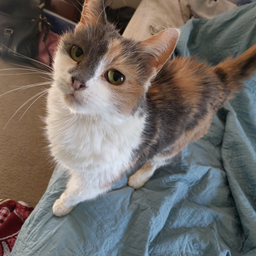
\includegraphics[width=8cm]{kitty}
\caption{Kitty}
\label{fig:kitty}
\end{figure}

\begin{figure}[H]
\centering
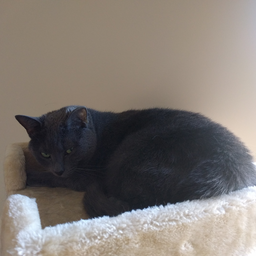
\includegraphics[width=8cm]{luna}
\caption{Luna}
\label{fig:luna}
\end{figure}

\begin{figure}[H]
\centering
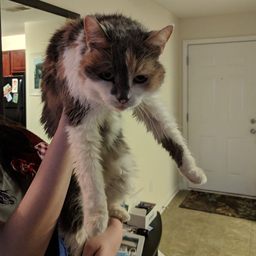
\includegraphics[width=8cm]{kitty2}
\caption{Kitty}
\label{fig:kitty}
\end{figure}


\begin{figure}[H]
\centering
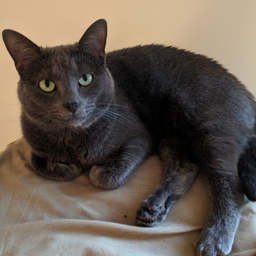
\includegraphics[width=8cm]{luna2}
\caption{{Luna}}
\label{fig:luna}
\end{figure}

The difference in features between these two cats are distinct, but they're not classifiably seperable as they're both cats.
I used an alpha value of 0.5 to mean shift this data set since grayscale values aren't close together. The results are shown below. Figure 6 represents the mean shifted data, and figure 5 represents the raw data of each 8x8 feature in a 256x256 image.

\begin{figure}[H]
\centering
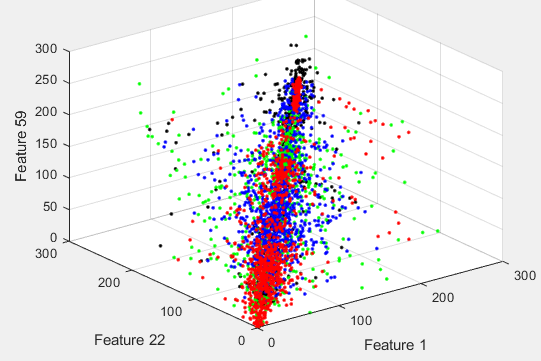
\includegraphics[width=8cm]{nomean}
\caption{{No mean cats}}
\label{fig:nmc}
\end{figure}

\begin{figure}[H]
\centering
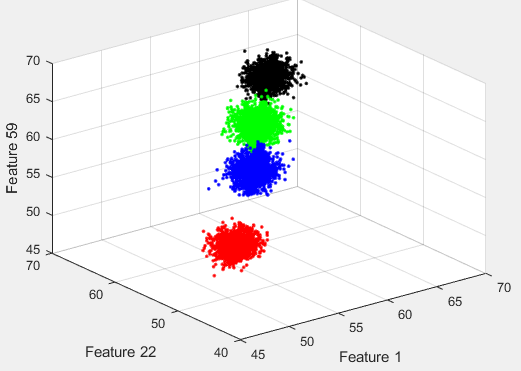
\includegraphics[width=8cm]{meanshifted}
\caption{{Mean shifted cats}}
\label{fig:msc}
\end{figure}


\subsection{Yogurt Lids}

This data set was a little tricky. The different between the lids was minimal. Color between 2 of the lids were very similar, and the shape of all of the lids were the same. These lids are shown below.\\

\begin{figure}[H]
\centering
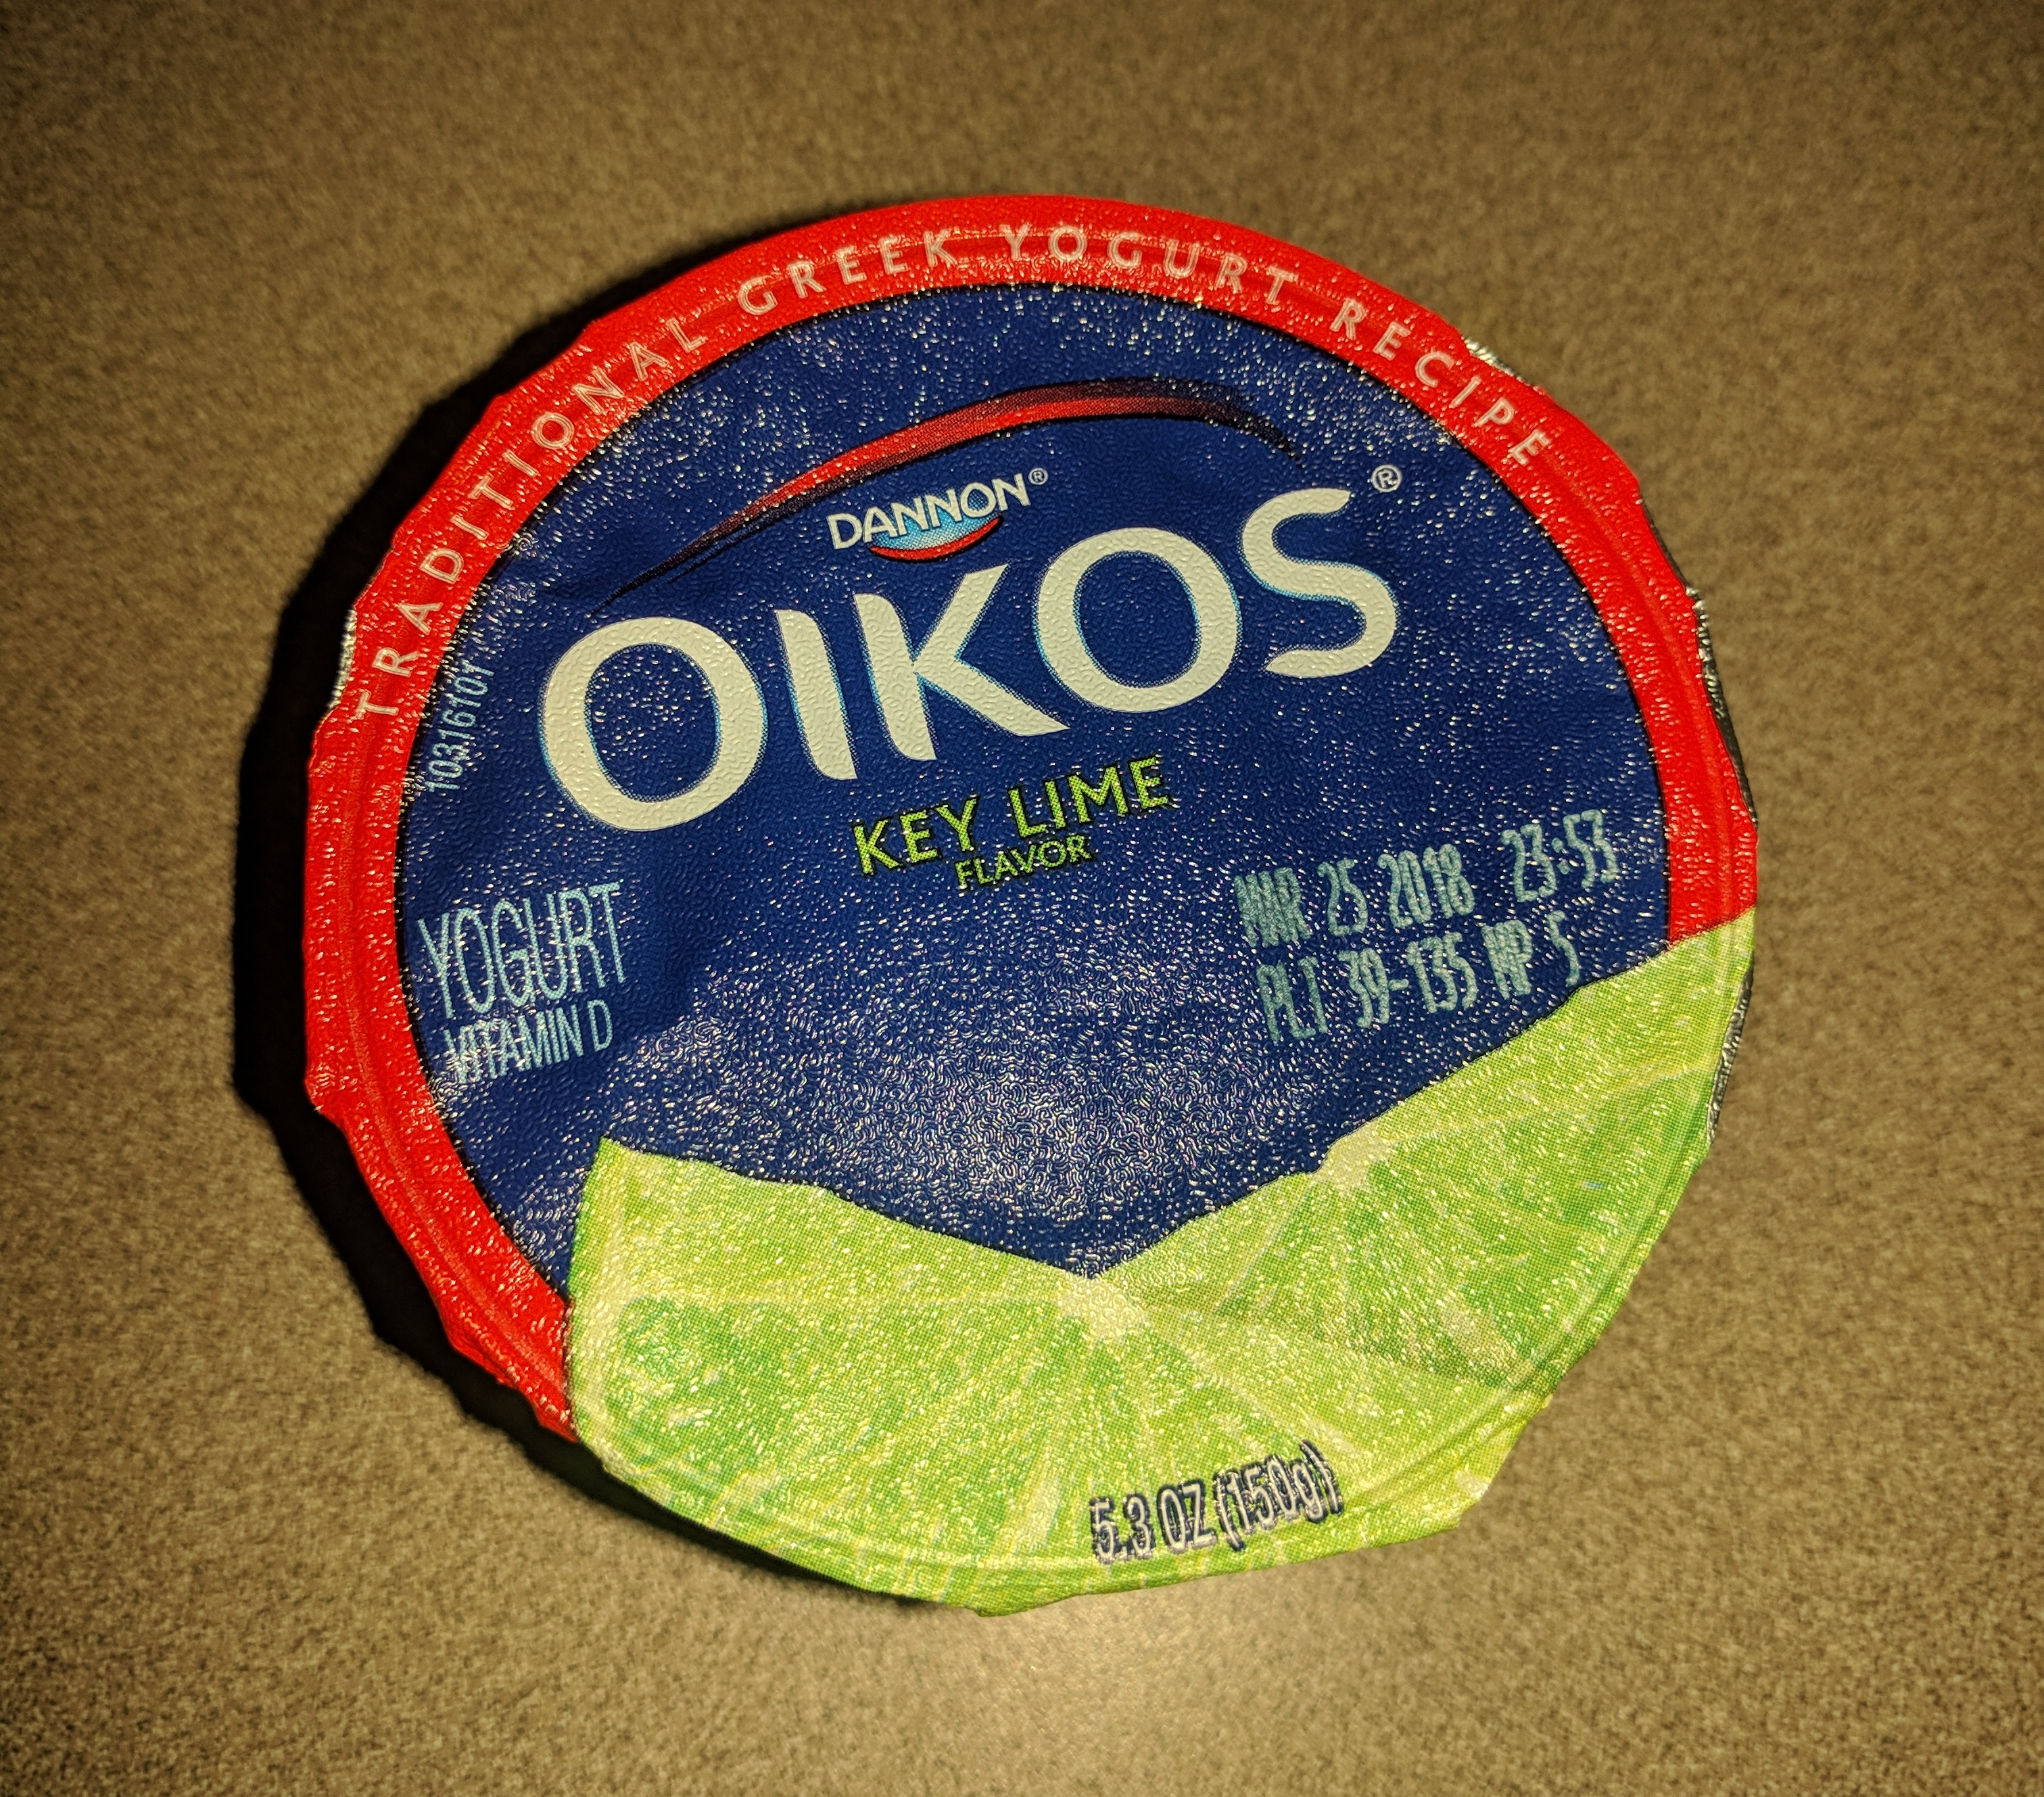
\includegraphics[width=8cm]{keylime}
\caption{{Keylime}}
\label{fig:keylime}
\end{figure}

\begin{figure}[H]
\centering
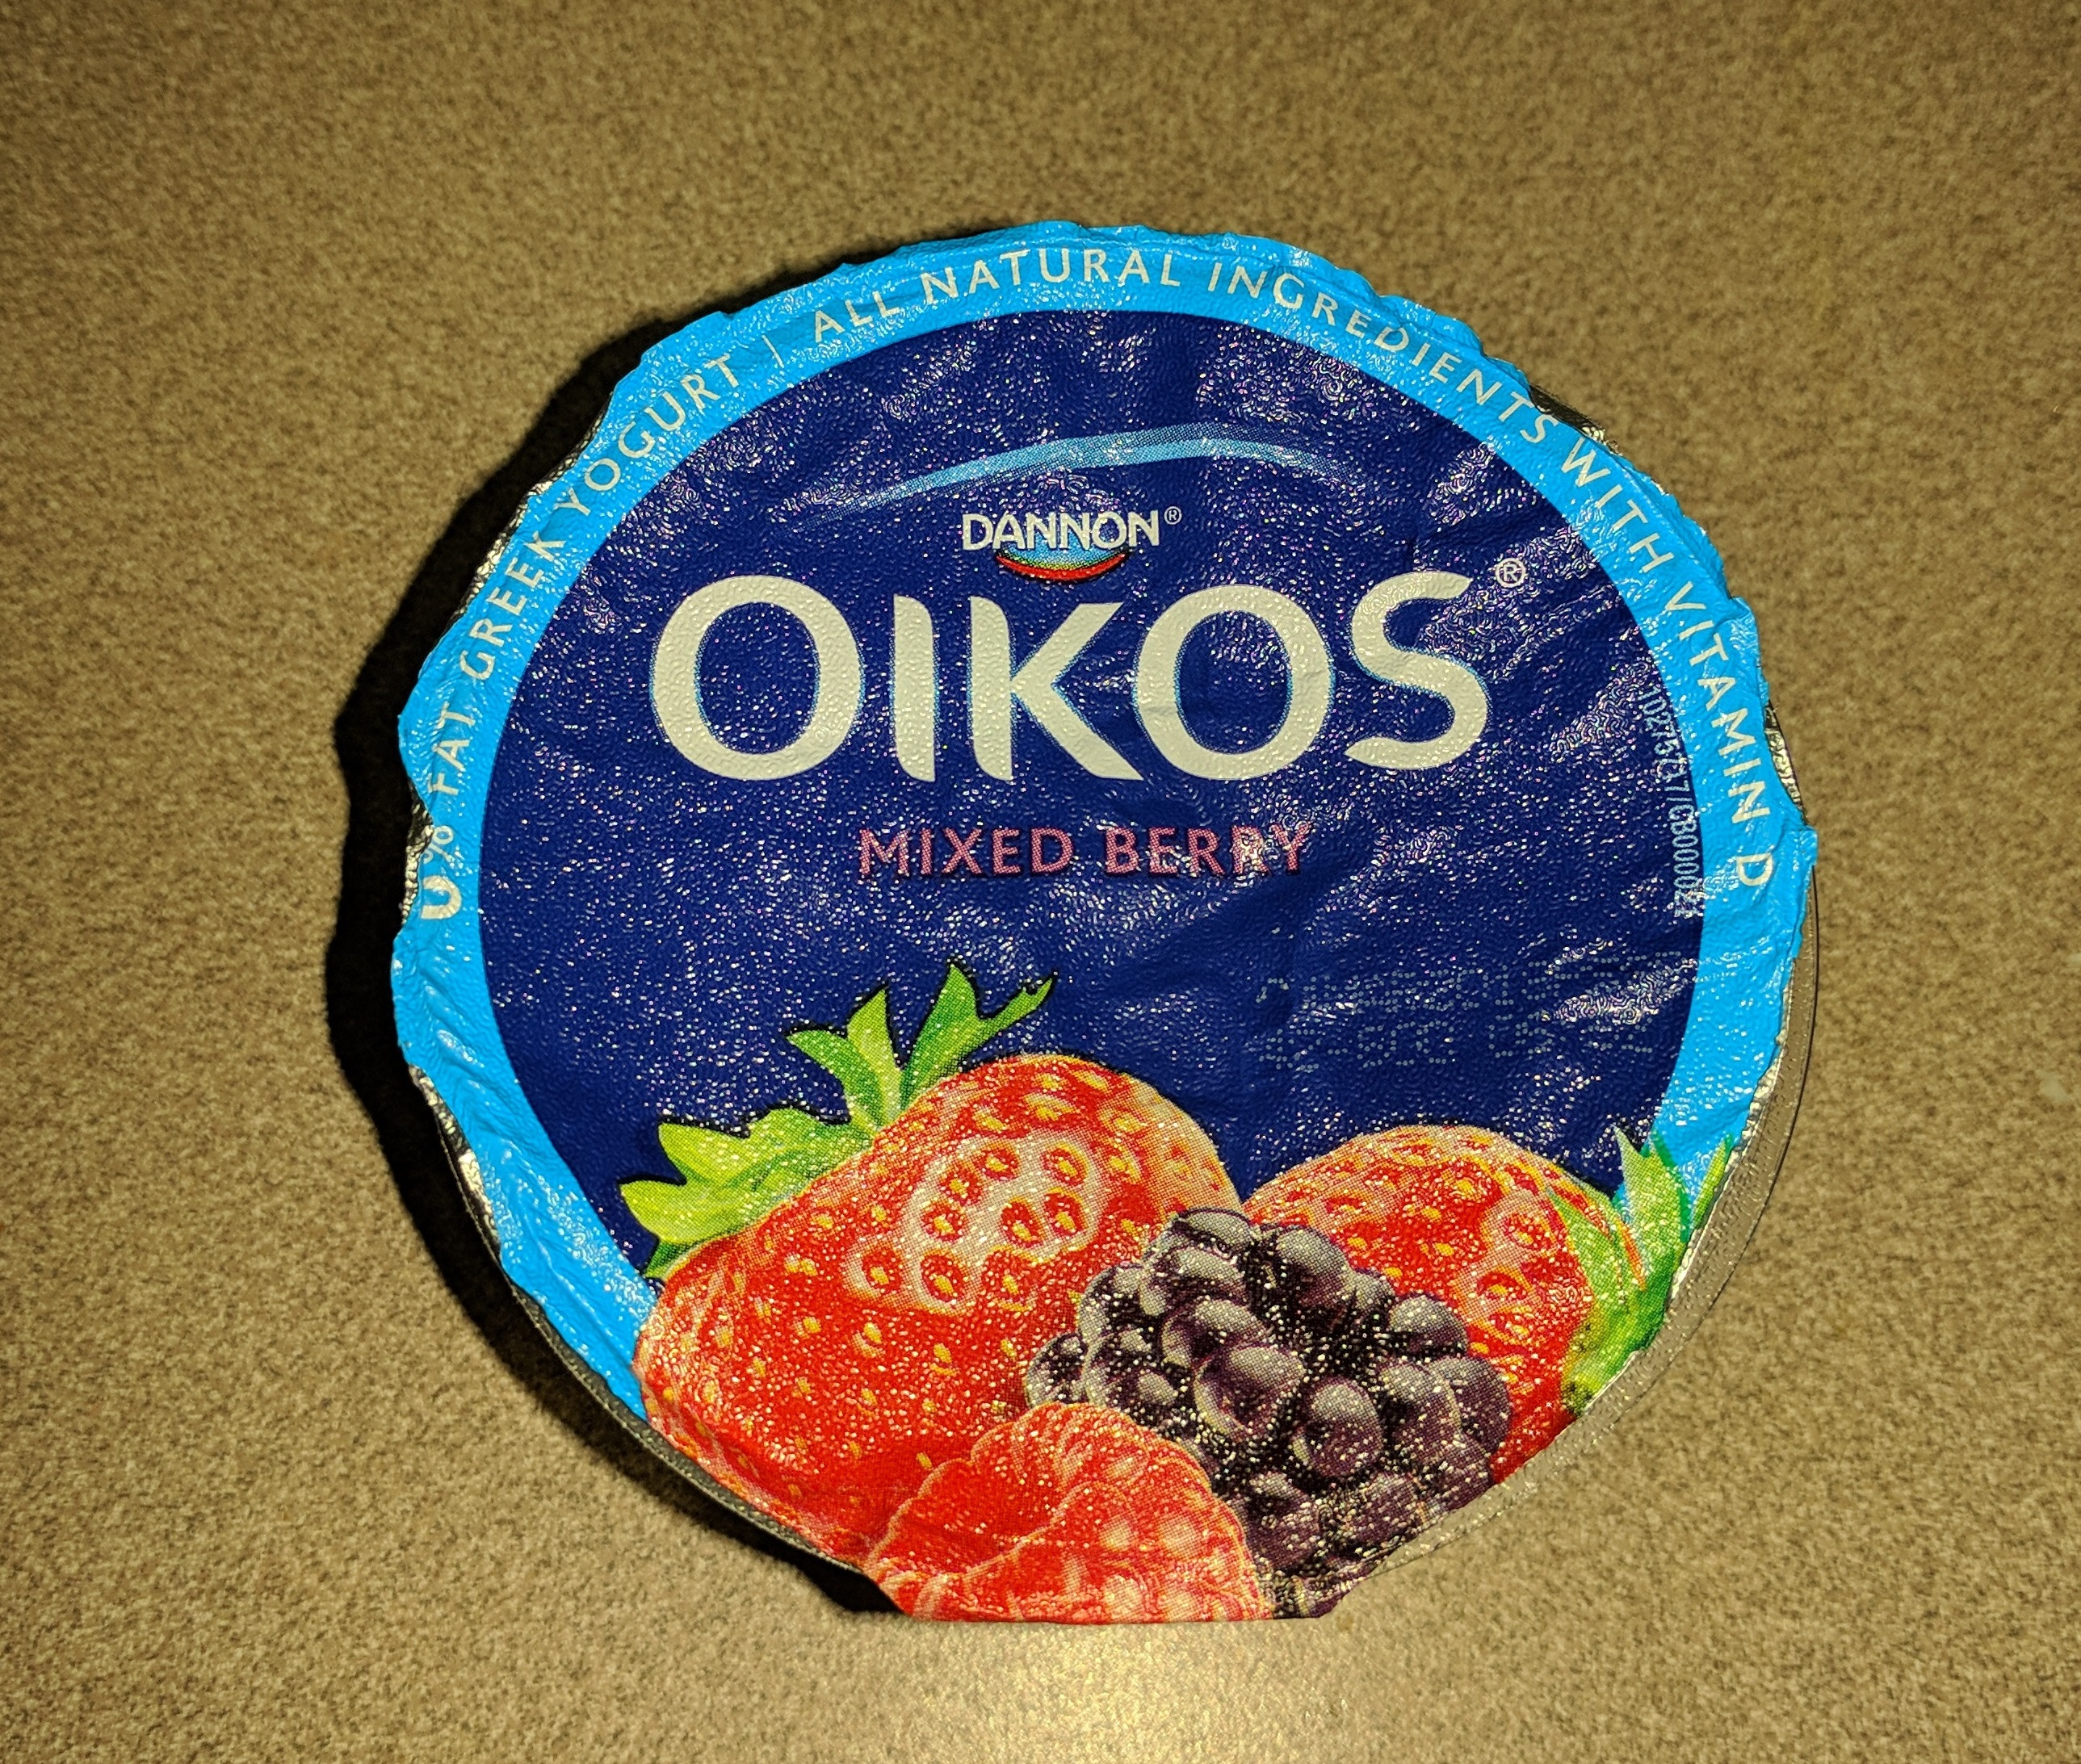
\includegraphics[width=8cm]{berry}
\caption{{Berry}}
\label{fig:berry}
\end{figure}

\begin{figure}[H]
\centering
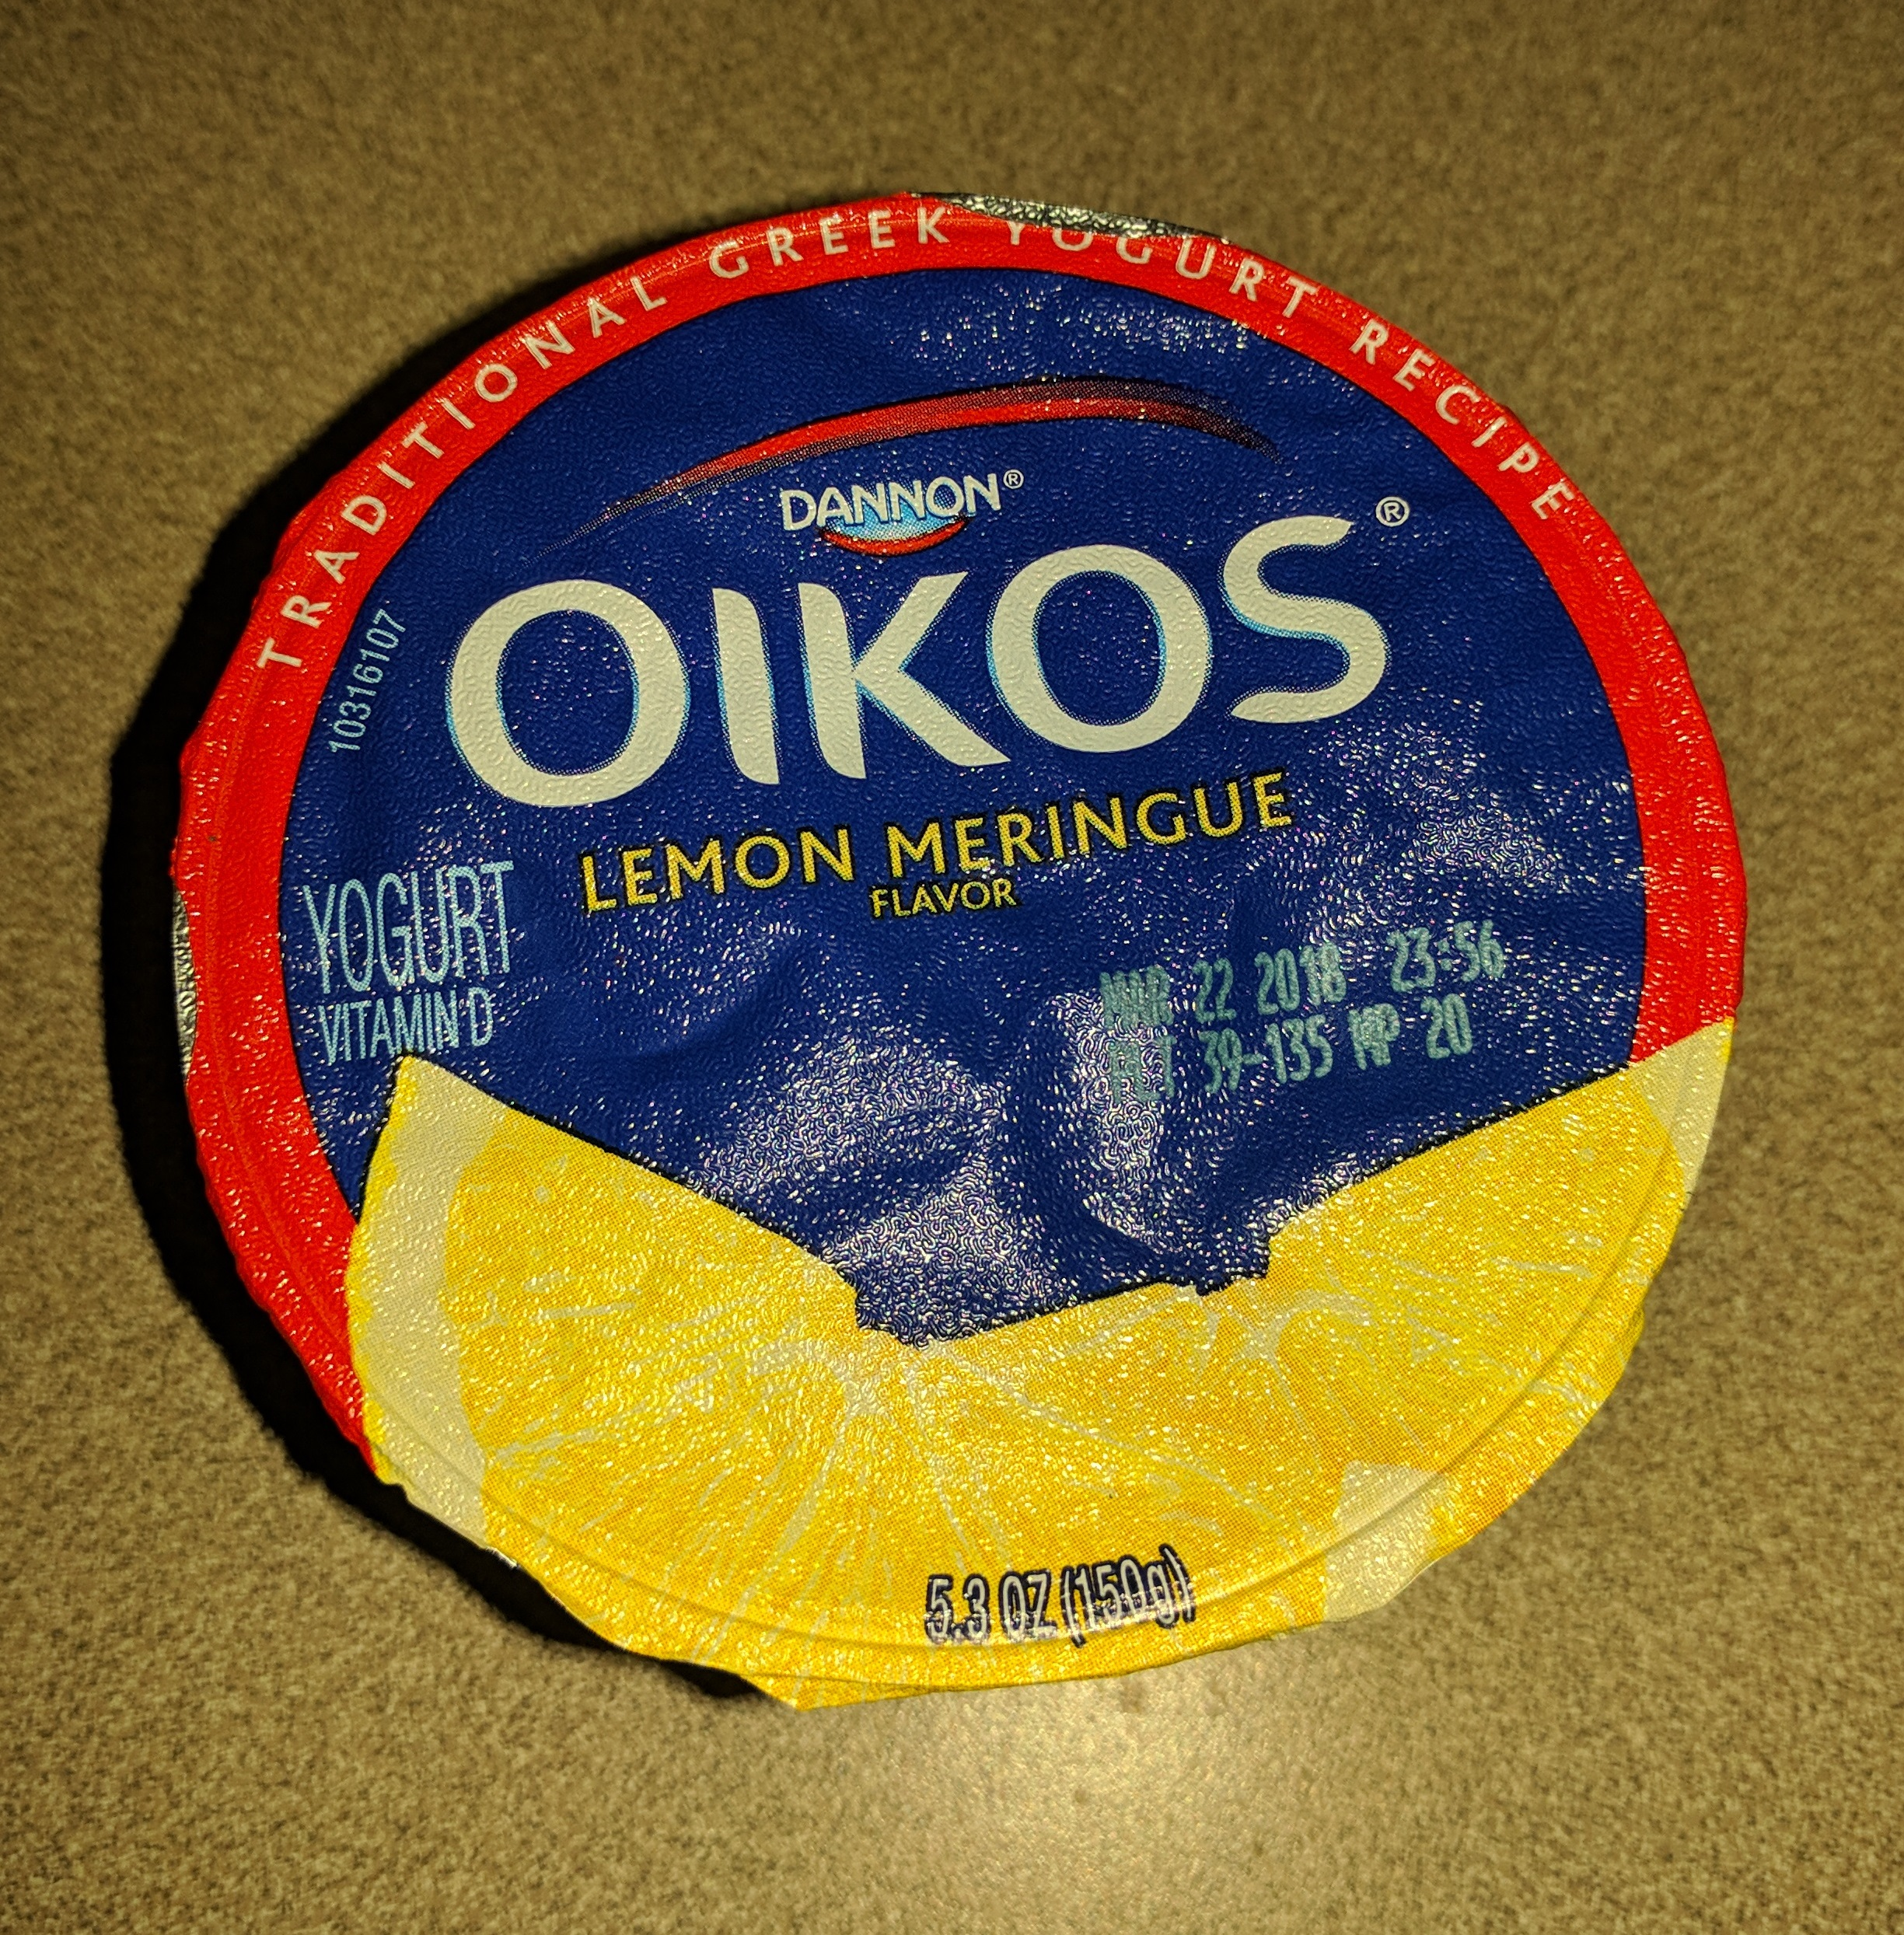
\includegraphics[width=8cm]{lemon}
\caption{{Lemon}}
\label{fig:lemon}
\end{figure}

\begin{figure}[H]
\centering
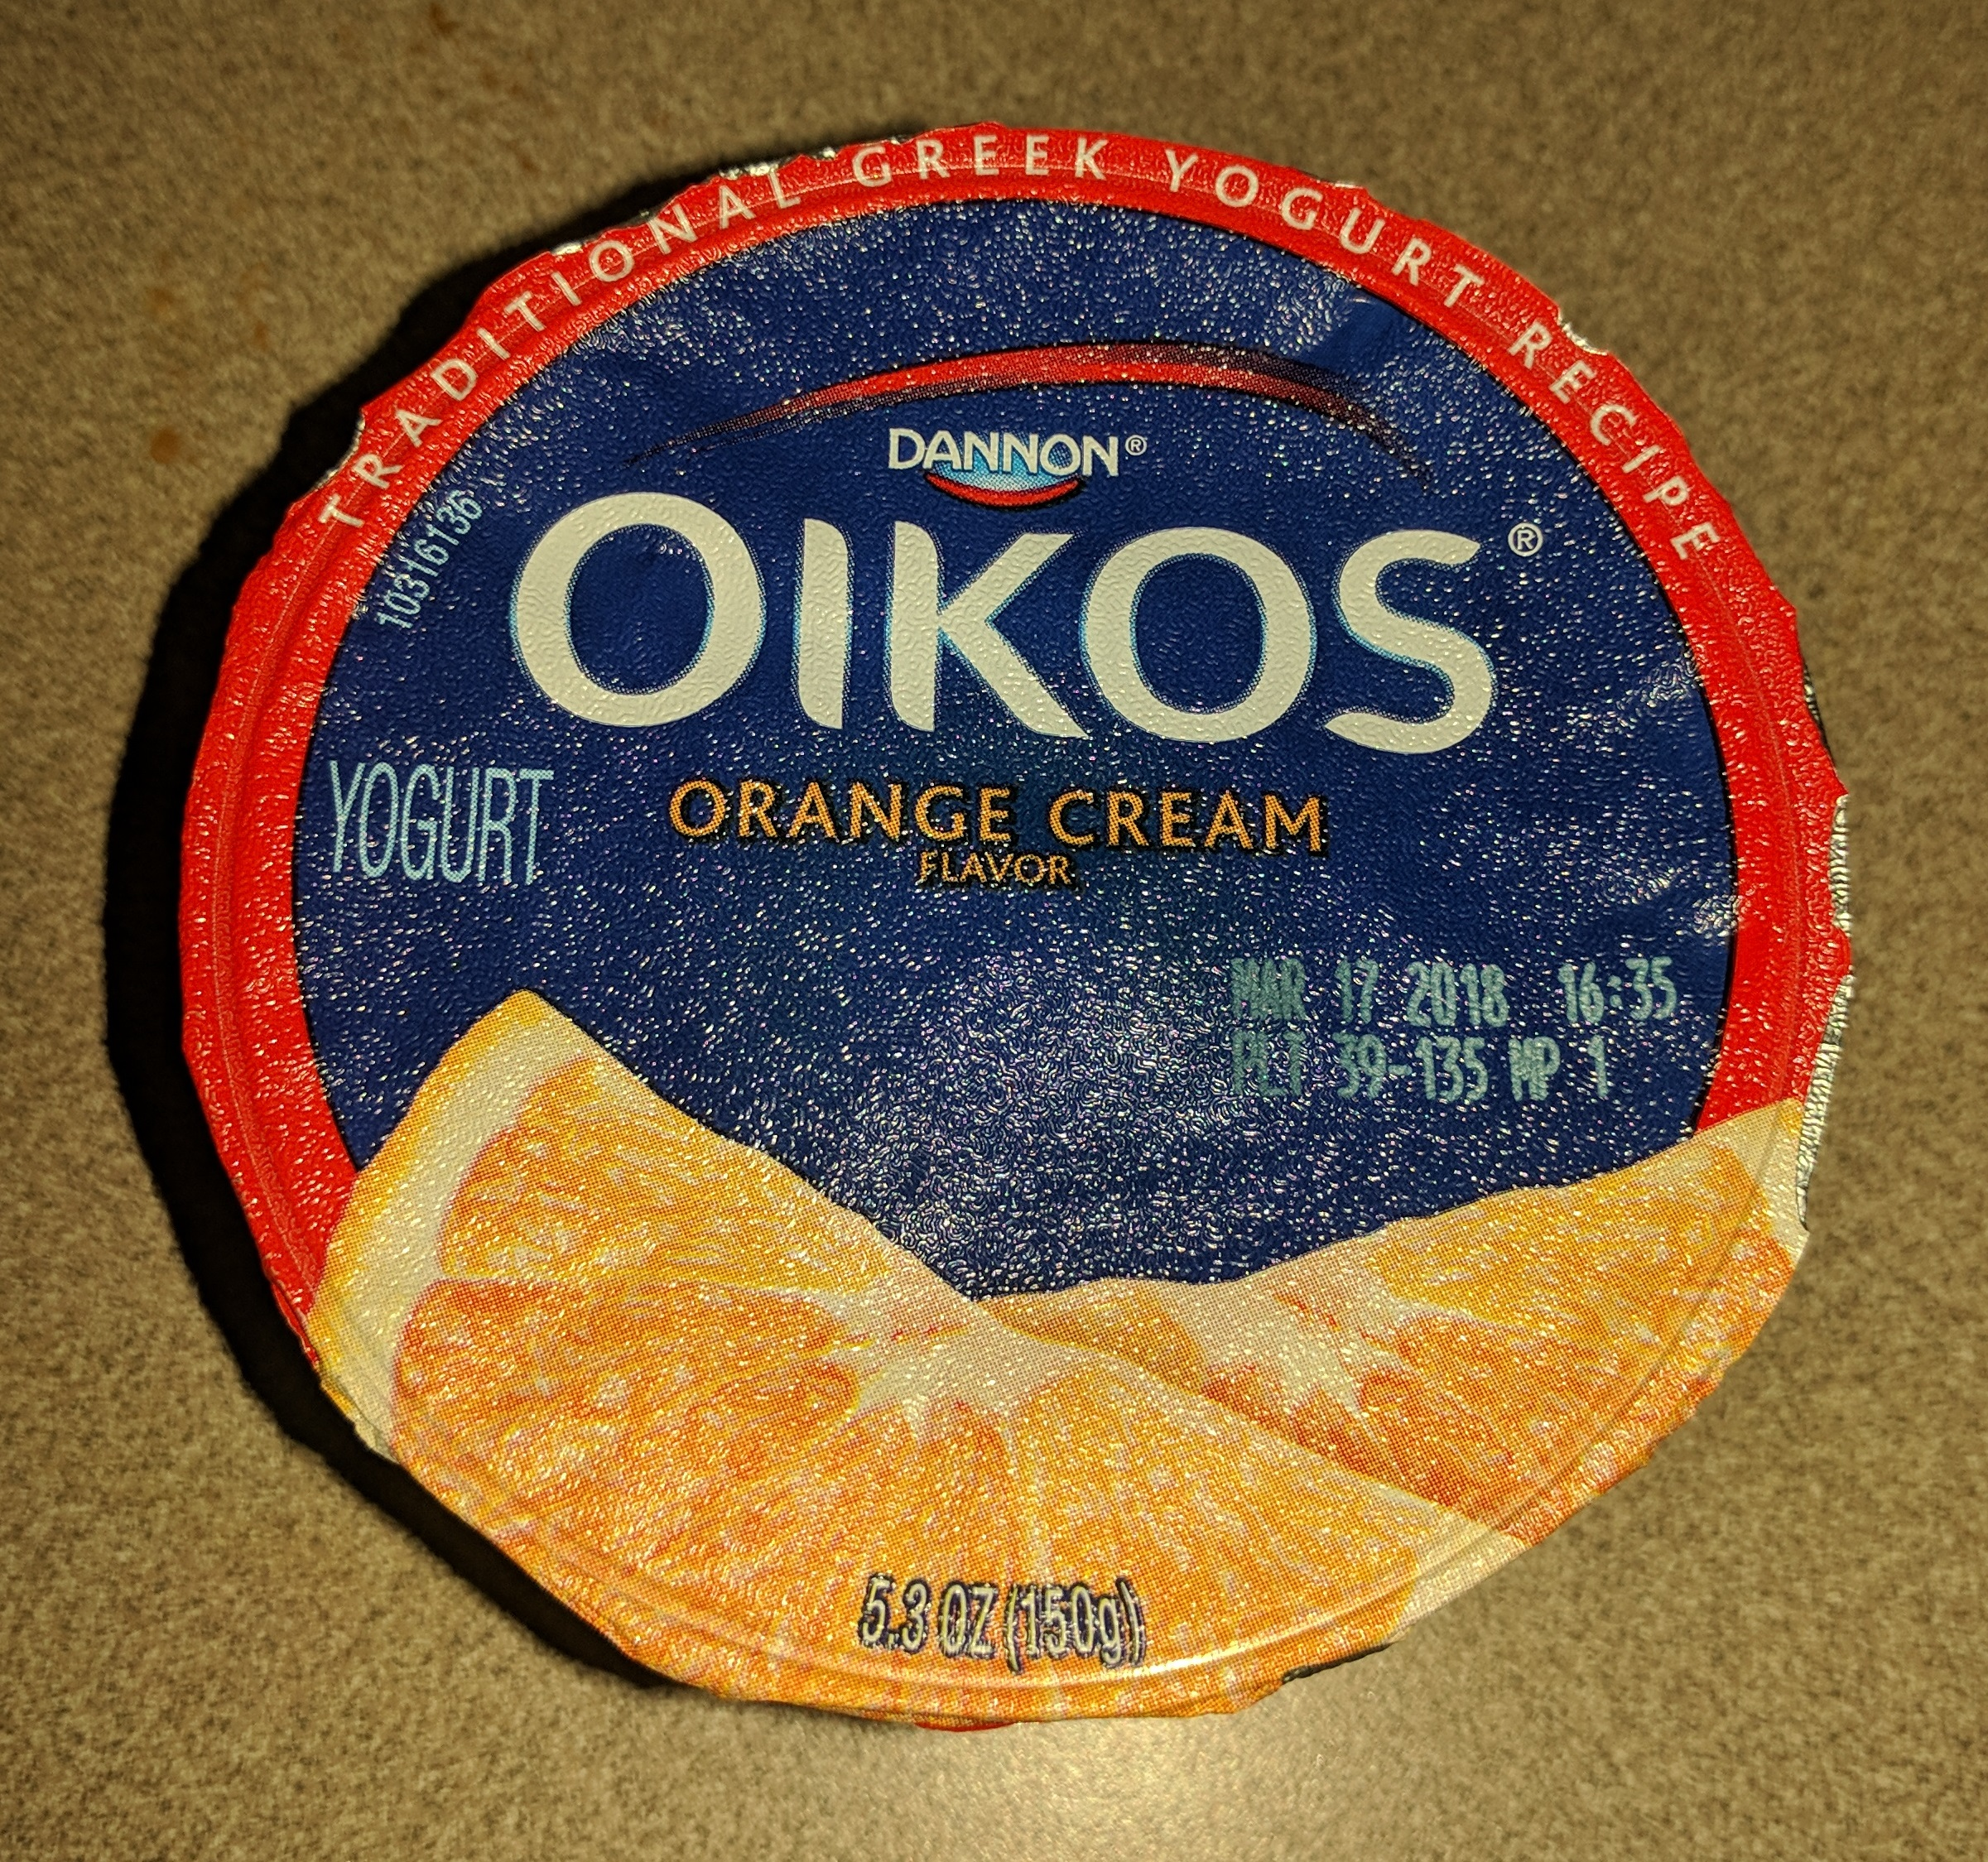
\includegraphics[width=8cm]{orange}
\caption{{Orange}}
\label{fig:orange}
\end{figure}


I had to use an alpha value of 5.00 with this data set, because the grayscale values of lemon and orange were very insignificantly different, even the image of the fruit on the front of the lid was nearly exact. Figure 11  below represents no mean shift, and figure 12 represents mean shifted with a value of 5.00

\subsection{Conclusion}

Making the distinction between yogurt lids is very difficult, they're the same shape and too similar in features. However, with a high enough mean shift it's possible to distinguish the two.

My cats on the other hand are very different in shape and color, making it easier to tell which cat is which. This data set used a low alpha value for mean shifts meaning it would not have a hard time during the training period.

\begin{figure}[H]
\centering
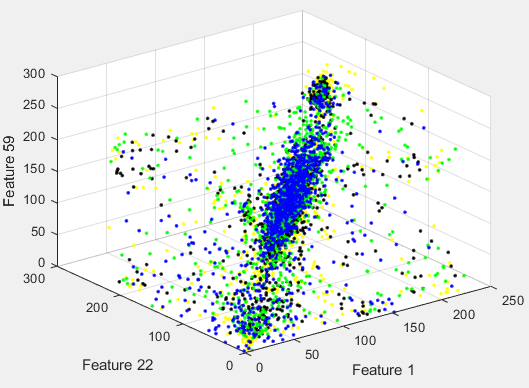
\includegraphics[width=8cm]{nomeanYogurt}
\caption{{No mean Yogurt}}
\label{fig:nmy}
\end{figure}


\begin{figure}[H]
\centering
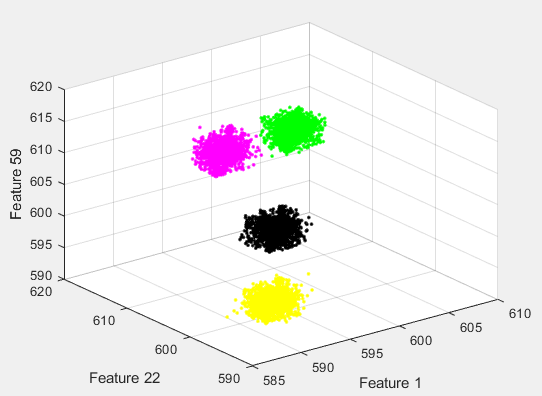
\includegraphics[width=8cm]{meanshiftedYogurt}
\caption{{Mean shifted Yogurt}}
\label{fig:msy}
\end{figure}


\section{Selecting Data Sets} 

The Cifar-10 dataset is a labeled subset of an 80 million image dataset. The batches contain 50,000 training images and 10,000 test images. The classes are mutually exclusive so there’s minimal potential for poor training with this dataset. The mutual exclusivity is the main point of my choice in this set. The training phase is the most important part for machine learning, and this extensive selection of tiny images will do the job very well. \\

\section{Introduction of the RHadoop System}
For this assignment I was tasked with implementing a distributed file system on linux for the purpose of big data processing in the final assignment. I used Hadoop 2.6 on Ubuntu 14.04. 

\subsection{Installing Java}
The Hadoop framework is written in java, so my first step was installing JDK version 1.7.0 on Ubuntu in my virtual machine.

\begin{figure}[H]
\centering
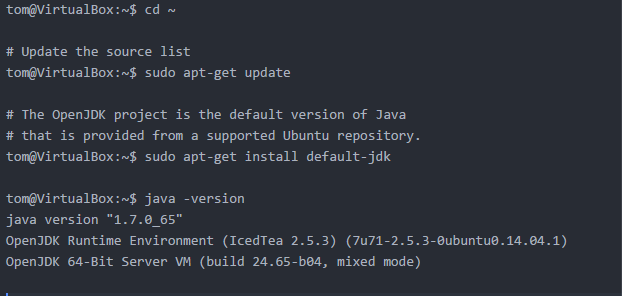
\includegraphics[width=12cm]{RH1}
\caption{Installing Java}
\label{fig:ij}
\end{figure}

\subsection{Adding a Dedicated Hadoop User}

\begin{figure}[H]
\centering
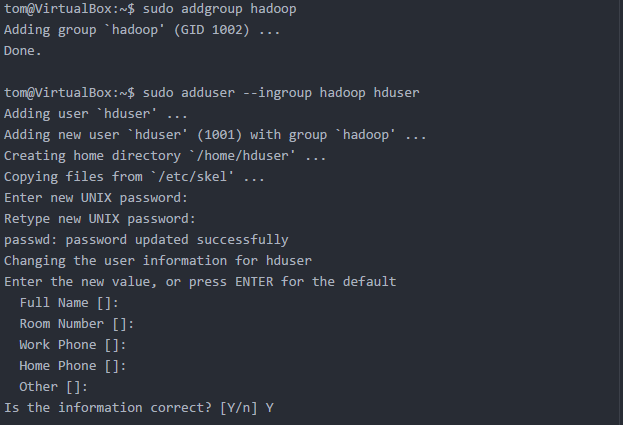
\includegraphics[width=12cm]{RH2}
\caption{Adding a dedicated Hadoop user.}
\label{fig:ij}
\end{figure}

\subsection{Installing SSH}

\begin{figure}[H]
\centering
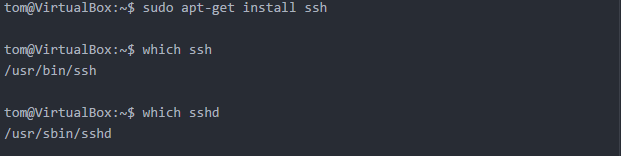
\includegraphics[width=12cm]{RH3}
\caption{Installing SSH.}
\label{fig:is}
\end{figure}

\subsection{Create and Setup SSH Certificates}

\begin{figure}[H]
\centering
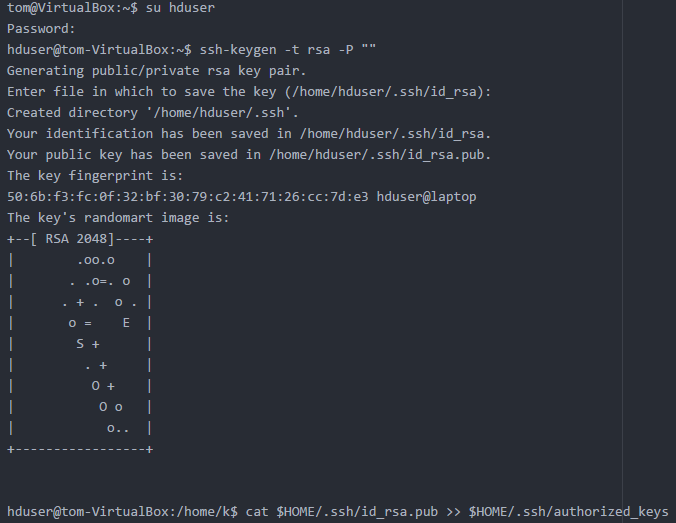
\includegraphics[width=12cm]{RH4}
\caption{Creating and setting up SSH Certificates.}
\label{fig:ij}
\end{figure}


\subsection{Installing Hadoop}

\begin{figure}[H]
\centering
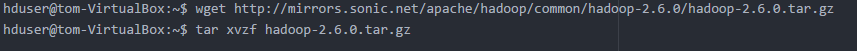
\includegraphics[width=12cm]{RH5}
\caption{Installing Hadoop.}
\label{fig:ij}
\end{figure}

\begin{figure}[H]
\centering
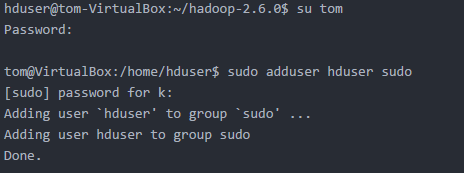
\includegraphics[width=12cm]{RH6}
\caption{Logging in as root user then adding hduser to sudo.}
\label{fig:ij}
\end{figure}

The hduser now has root privilege. We can now move the Hadoop installation to the /usr/local/hadoop directory.

\begin{figure}[H]
\centering
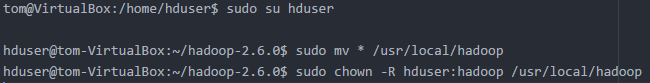
\includegraphics[width=12cm]{RH7}
\caption{Moving Hadoop installation.}
\label{fig:ij}
\end{figure}


\section{Configuring Hadoop Files}


\subsection{~/.bashrc}

I needed to set some hadoop variables inside the ~/.bashrc file. Such as the hadoop install path and Java's home.

\begin{figure}[H]
\centering
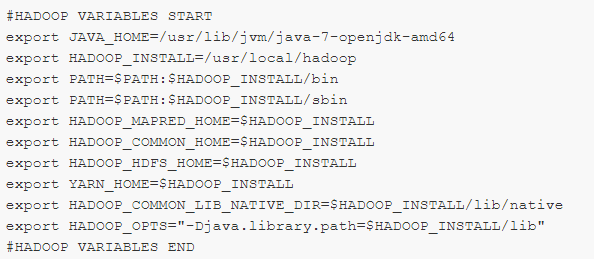
\includegraphics[width=12cm]{RH8}
\caption{Appended lines}
\label{fig:ij}
\end{figure}


\subsection{/usr/local/hadoop/etc/hadoop/hadoop-env.sh}

\begin{figure}[H]
\centering
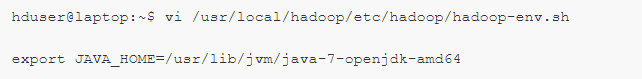
\includegraphics[width=12cm]{RH10}
\caption{Setting JAVA\_HOME by modifying hadoop-env.sh}
\label{fig:ij}
\end{figure}


\subsection{/usr/local/hadoop/etc/hadoop/core-site.xml:}

\begin{figure}[H]
\centering
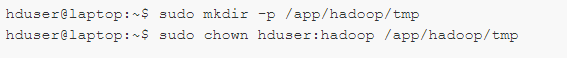
\includegraphics[width=12cm]{RH11}
\label{fig:ij}
\end{figure}

\begin{figure}[H]
\centering
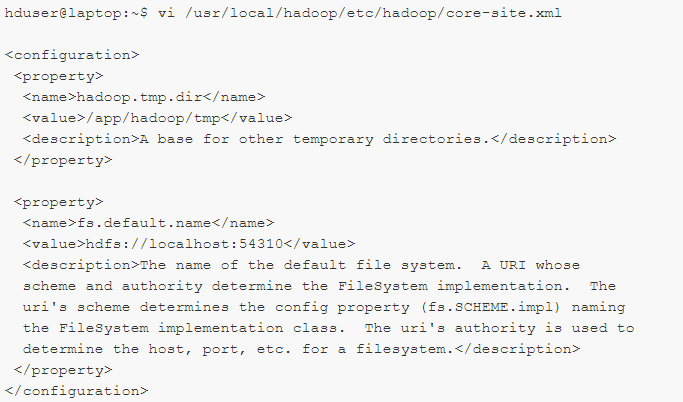
\includegraphics[width=12cm]{RH12}
\caption{Changing Hadoop config that it uses when starting up.}
\label{fig:ij}
\end{figure}

\subsection{/usr/local/hadoop/etc/hadoop/mapred-site.xml}

The mapred-site.xml file is used to specify which framework is being used for MapReduce. I needed to enter Figure 23's content in between the <configuration></configuration> tag

\begin{figure}[H]
\centering
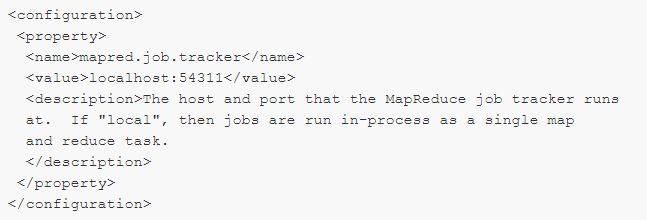
\includegraphics[width=12cm]{RH13}
\caption{Changing mapred-site.xml.}
\label{fig:ij}
\end{figure}

\subsection{/usr/local/hadoop/etc/hadoop/hdfs-site.xml}

The /usr/local/hadoop/etc/hadoop/hdfs-site.xml file needs to be configured for each host in the cluster that is being used.  It's used to specify the directories which will be used as the namenode and the datanode on that host.  I needed to enter Figure 24's content in between the <configuration></configuration> tag

\begin{figure}[H]
\centering
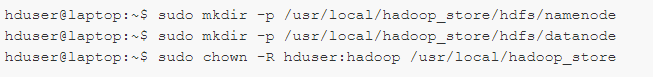
\includegraphics[width=12cm]{RH14}
\label{fig:ij}
\end{figure}

\begin{figure}[H]
\centering
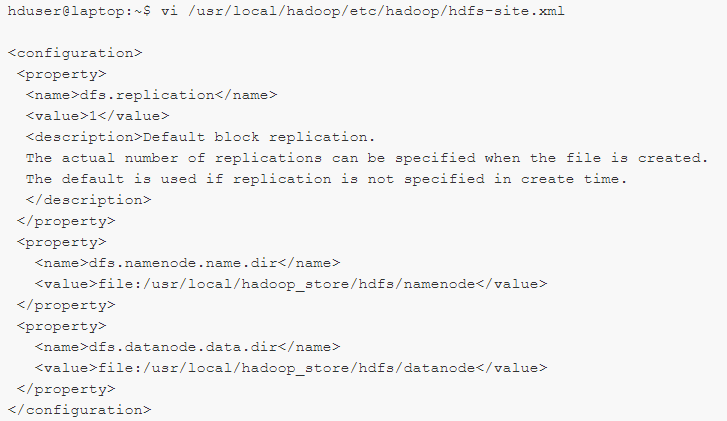
\includegraphics[width=12cm]{RH15}
\caption{Changing hdfs-site.xml.}
\label{fig:ij}
\end{figure}

\section{Formatting the Hadoop Filesystem}

The Hadoop file system needs to be formatted so that I could start using it. The format command was issued with write permission since it creates current directory under /usr/local/hadoop\_store/hdfs/namenode folder. This command was executed before using Hadoop. 

\begin{figure}[H]
\centering
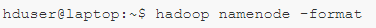
\includegraphics[width=12cm]{RH16}
\caption{Format Hadoop command.}
\label{fig:ij}
\end{figure}

\section{Starting Hadoop}

\begin{figure}[H]
\centering
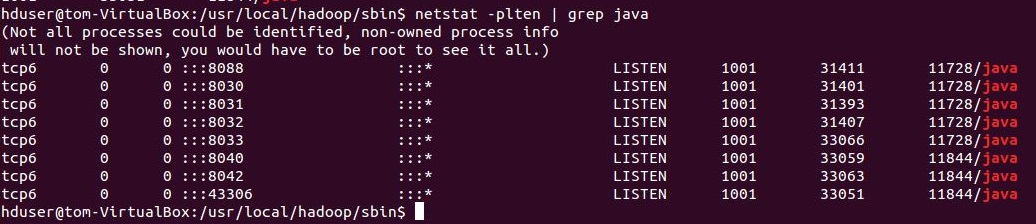
\includegraphics[width=12cm]{proof.JPG}
\caption{Netstat command.}
\label{fig:netstat}
\end{figure}

:::8088 in this cluster is the host node. The other nodes are all slaves. Since :::8088 is the host of the node cluster, once Hadoop is started the web interface can be accessed at localhost:8088. This web interface details the current state of the Hadoop Distributed File System. You can view current working jobs that the file system is running, and manage the nodes individually. This interface is shown below in figure 27. My Node Cluster has a total of 8GB memory.

\begin{figure}[H]
\centering
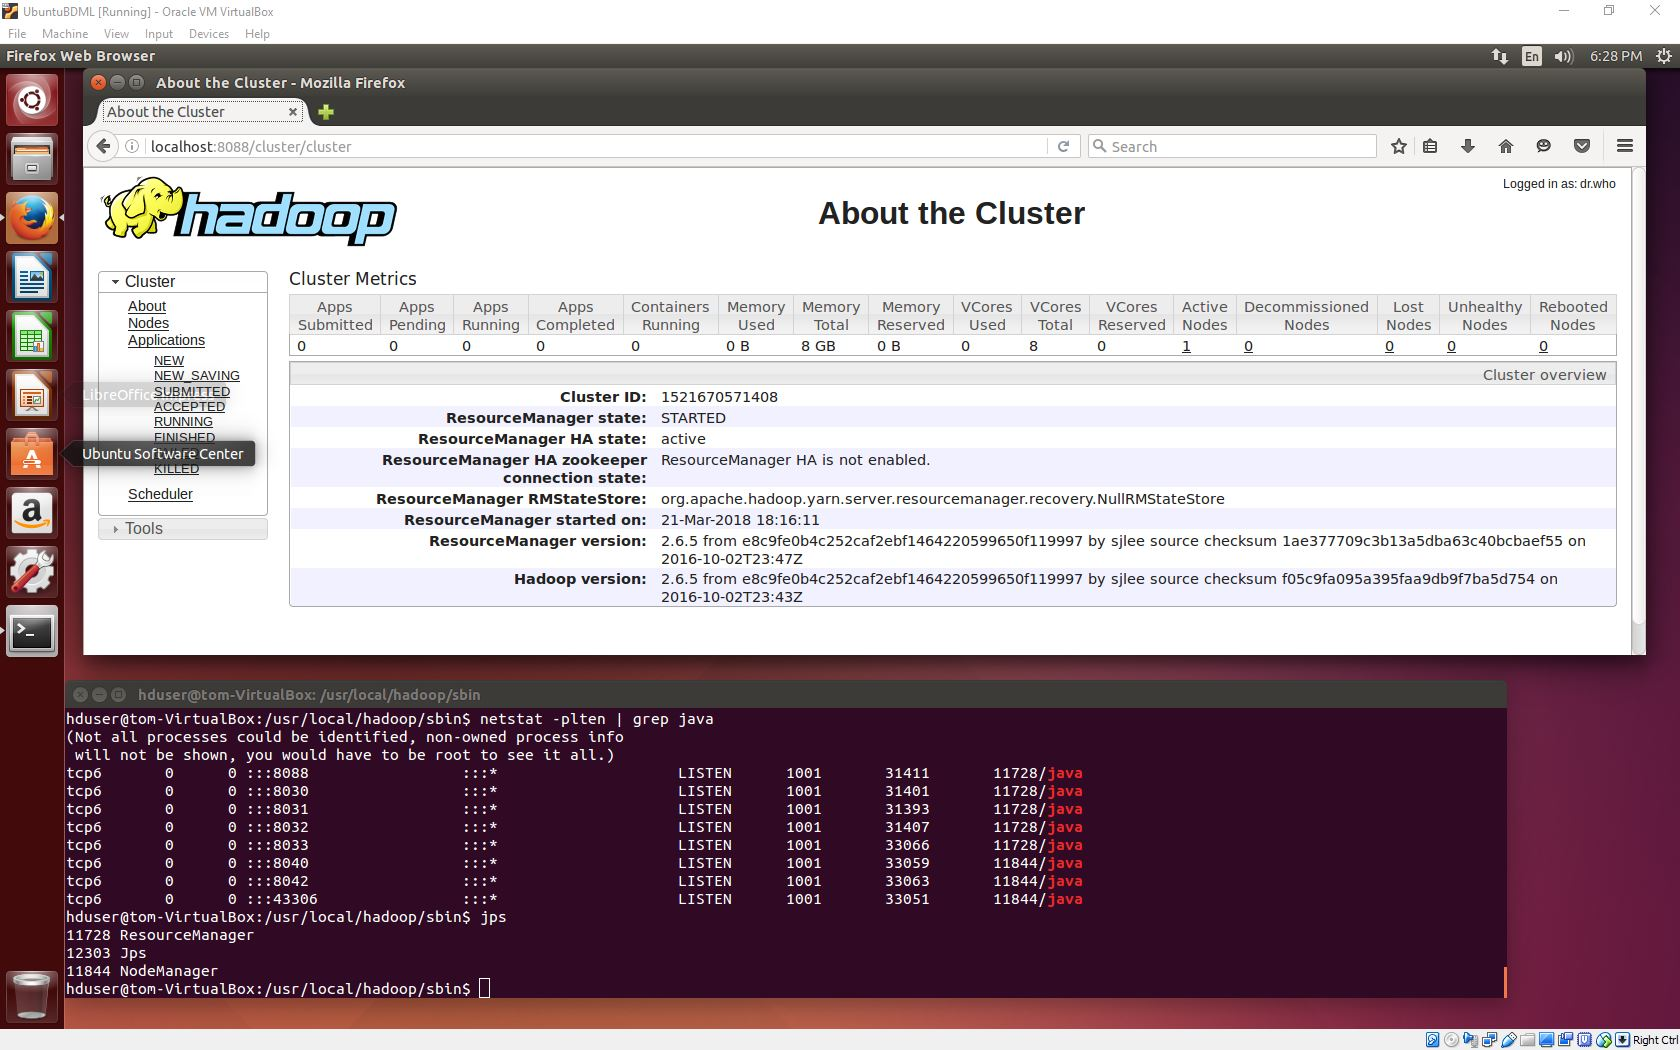
\includegraphics[width=12cm]{moreproof.JPG}
\caption{Hadoop web interface.}
\label{fig:one}
\end{figure}

\section{Machine Learning}

\subsection{Introduction}
The last step in this class is to introduce a machine learning algorithm and use the generated data on it. This machine learning algorithm will be fed with my two datasets of four images each and test it's Out-Of-Bucket (OOB) estimation to determine how well the machine has learned these images.

\subsection{Choosing a Machine Learning Model}
With a variety of machine learning models to choose from. In this assignment we will pursue a supervised learning model that uses inferences from the dataset to predict future knowledge. Choosing a supervised learning models means that the data is labeled, and the desired output is to match those labels. We will also be using decision trees and random forest models for our supervised learning techniques. Random forest is a good choice for my datasets because my data contains several classes.

\subsection{Labeling and Shuffling}
Recall Figure's 1 through 4, two pictures of Kitty and two pictures of Luna. We expressed these images as data in csv files, an 8x8 grid of pixels is an observation, and every pixel in that grid is a feature. One image can be defined as a 256x256 image converted into 1024 observations containing 64 features. This data was labeled by me, a new 65th column was added to each observation. These labels were expressed in the numbers one to four, one and two represented the two pictures of Luna, three and four represented the two pictures of Kitty. The same method was then applied to the four different yogurt lids. Since we're not comparing cats to yogurt lids, the yogurt labels were also one through four. Now the data needs to be consolidated into one data file instead of four different files. The data also needs to be shuffled, to confuse the machine learning algorithm during testing phase. These were done in MatLab with a very simple script shown in figure 28.

\begin{figure}[H]
\centering
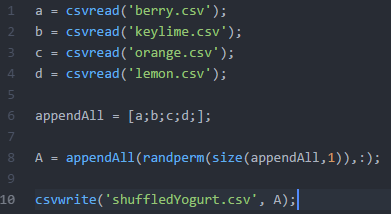
\includegraphics[width=5.0in]{matlabfile}
\caption{MatLab Script.}
\label{fig:mls}
\end{figure}

\subsection{Cat Comparisons: Kitty or Luna?}
The data has been labelled, appended, and shuffled at this point. Now we can start feeding in these two datasets into our machine learning algorithm. First we'll take a look at the machine's evaluation of the data in decision tree form. In this next figure, figure 29, the diagram will look like an upside-down tree. At the root of this tree is a feature that contributed the most in determining the location of the decision tree's split.

\begin{figure}[H]
\centering
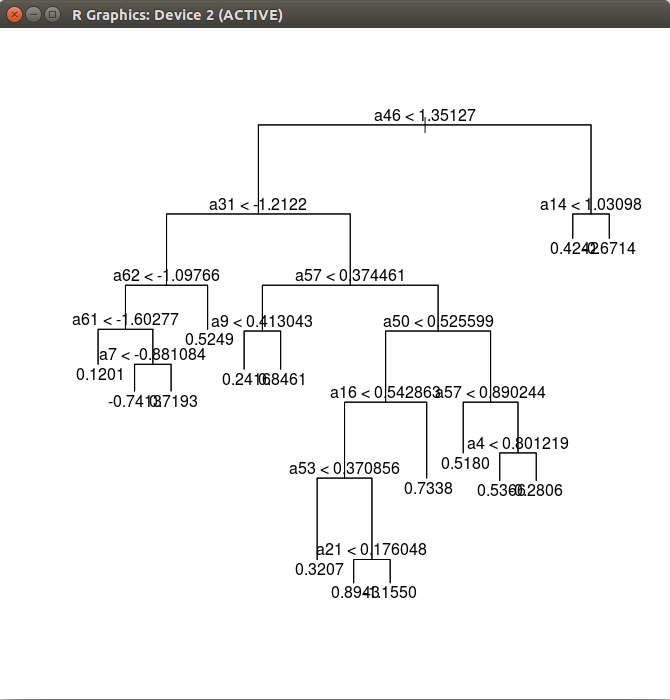
\includegraphics[width=5.0in]{catplot4}
\caption{Decision tree for the cat dataset Script.}
\label{fig:dtcd}
\end{figure}

We can see that feature 46 contributed the most to the location of the split. Any values in the data that are less than 1.35127 are split to the left, else it's split to the right. So on and so forth until the algorithm stops splitting and we're left with the leaves. The next five figures are results of the decision tree represented in other forms.

\begin{figure}[H]
\centering
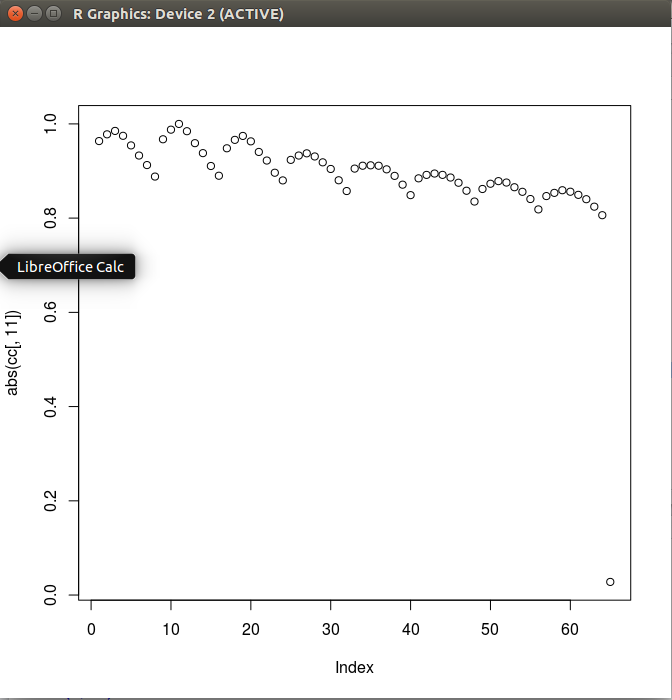
\includegraphics[width=5.0in]{catplot1}
\caption{Decision tree for the cat dataset Script.}
\label{fig:dtcd}
\end{figure}

\begin{figure}[H]
\centering
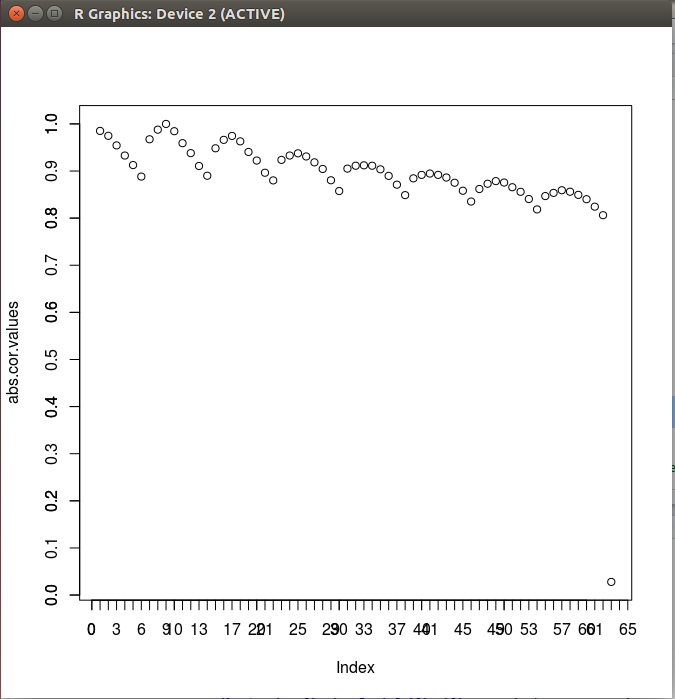
\includegraphics[width=5.0in]{catplot2}
\caption{Decision tree for the cat dataset Script.}
\label{fig:dtcd}
\end{figure}

\begin{figure}[H]
\centering
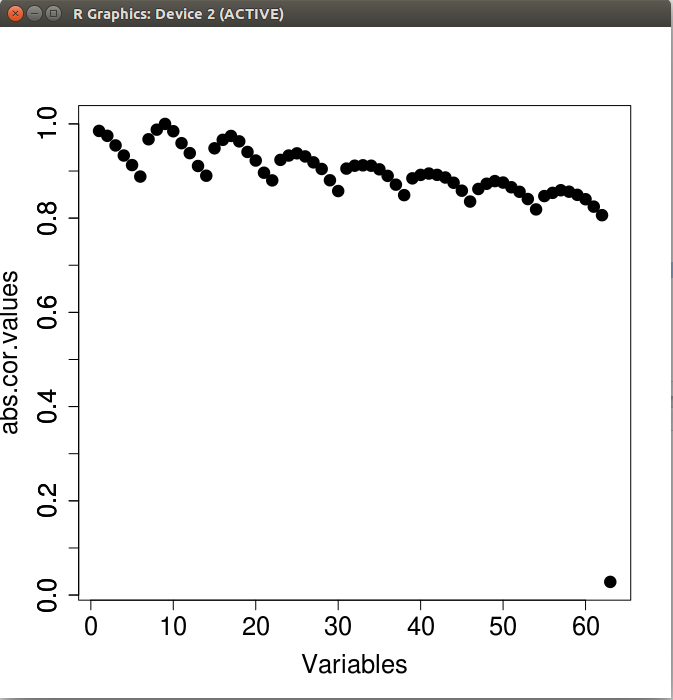
\includegraphics[width=5.0in]{catplot3}
\caption{Decision tree for the cat dataset Script.}
\label{fig:dtcd}
\end{figure}

\begin{figure}[H]
\centering
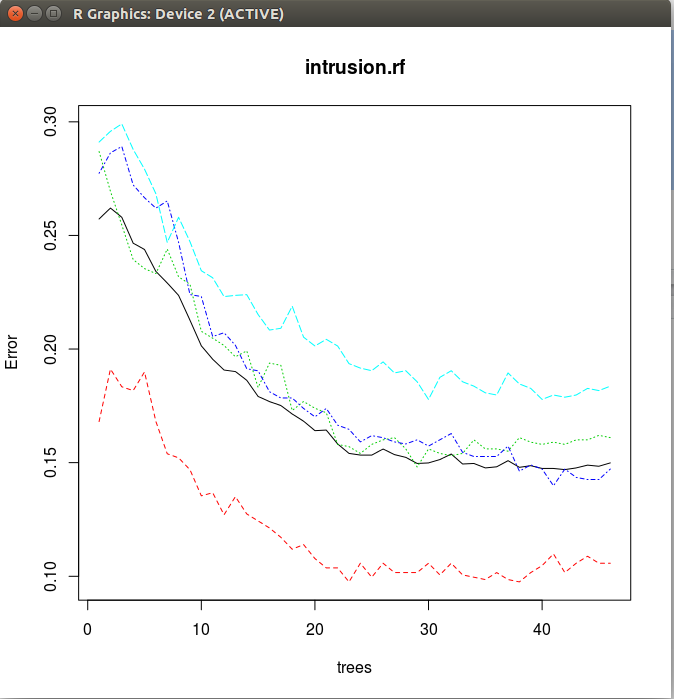
\includegraphics[width=5.0in]{catplot5}
\caption{Decision tree for the cat dataset Script.}
\label{fig:dtcd}
\end{figure}

\begin{figure}[H]
\centering
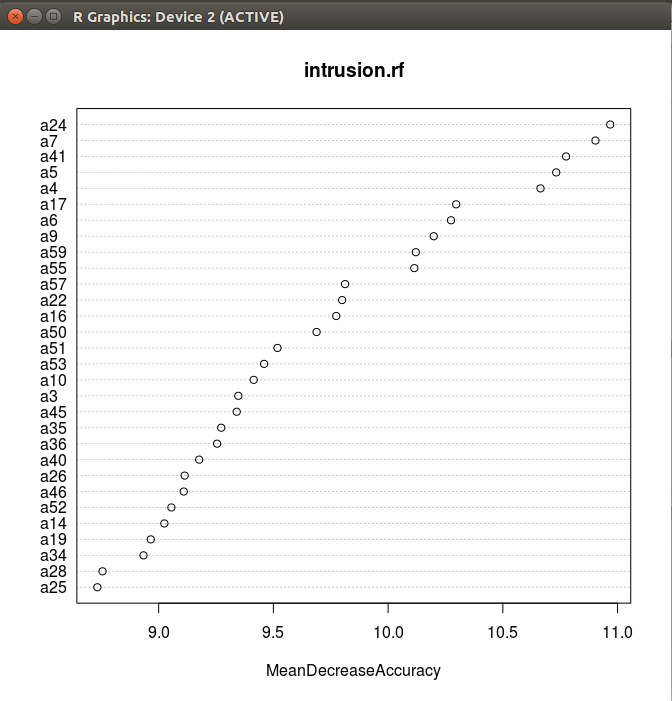
\includegraphics[width=5.0in]{catplot6}
\caption{Decision tree for the cat dataset Script.}
\label{fig:dtcd}
\end{figure}


 In the next three figures I'll show the random forest model's results of the cat dataset. Each of these figures have a different amount of trees, one is 250, one is 500, and the last is 1000. The differences between these trees should be substantial, however they're all within 1\% OOB estimate range of eachother.

\begin{figure}[H]
\centering
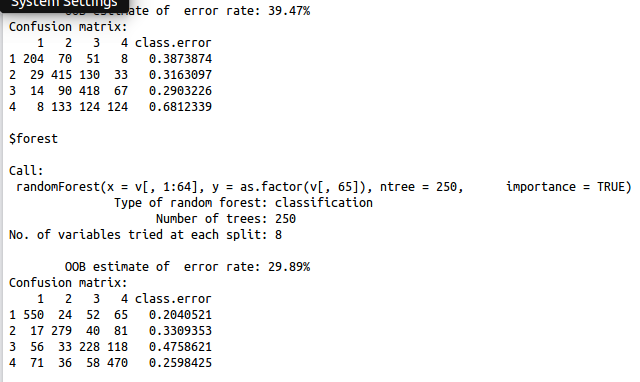
\includegraphics[width=5.0in]{catOOB250}
\caption{OOB where ntree = 250.}
\label{fig:oob1}
\end{figure}

\begin{figure}[H]
\centering
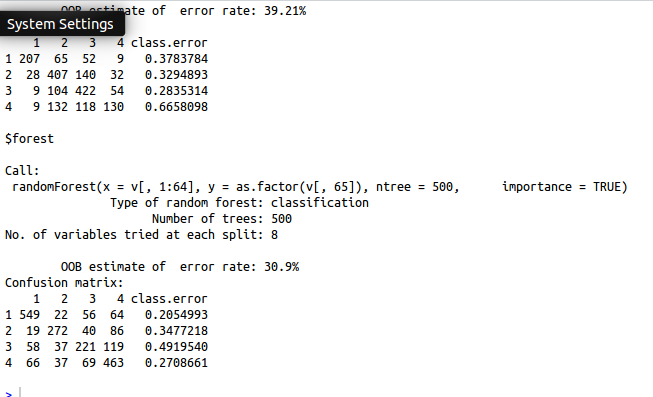
\includegraphics[width=5.0in]{catOOB500}
\caption{OOB where ntree = 500.}
\label{fig:oob2}
\end{figure}

\begin{figure}[H]
\centering
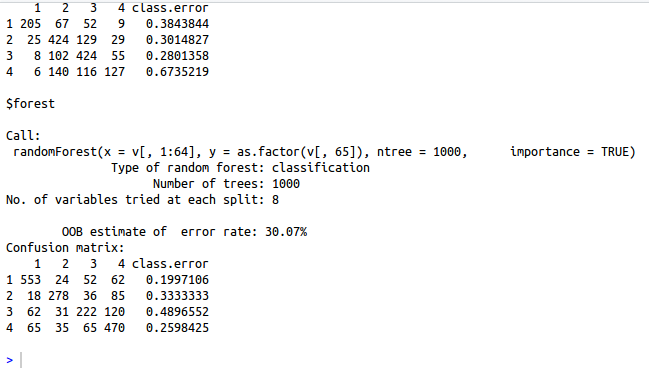
\includegraphics[width=5.0in]{catOOB1000}
\caption{OOB where ntree = 1000.}
\label{fig:oob3}
\end{figure}

Of the above three random forests 250 trees seems to be the best with a 70.11\% in accuracy.

\subsection{Which Flavor of Yogurt Should I Eat?}
After labelling, appending, and shuffling the data of the 4 different yogurt lids we're ready to pass the data into the random forests and decision trees as we have with the cat dataset. 

\begin{figure}[H]
\centering
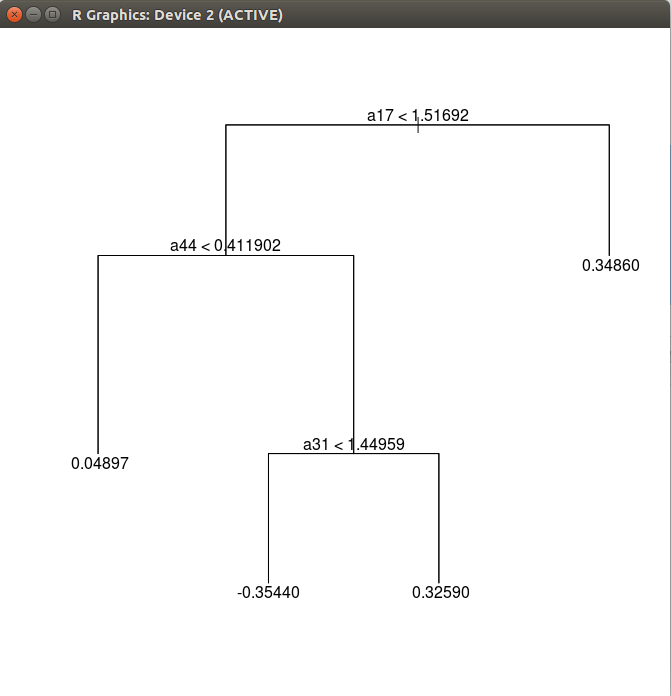
\includegraphics[width=5.0in]{yogurtplot4}
\caption{Decision tree for the yogurt dataset Script.}
\label{fig:dtyd}
\end{figure}

You may be thinking that this decision tree has much less branching than the cat dataset. This can be explained as less levels of decisions. If you can recall figures seven through eleven, the yogurt lids have far less differences between each other than the differences between the four cat images. In this decision tree, feature a17 has the most influence on the location of the splitting of the tree. Again, values less than 1.51692 are branched to the left, while the greater values are branched to the right. The next five figures are results of the decision tree represented in other forms.

\begin{figure}[H]
\centering
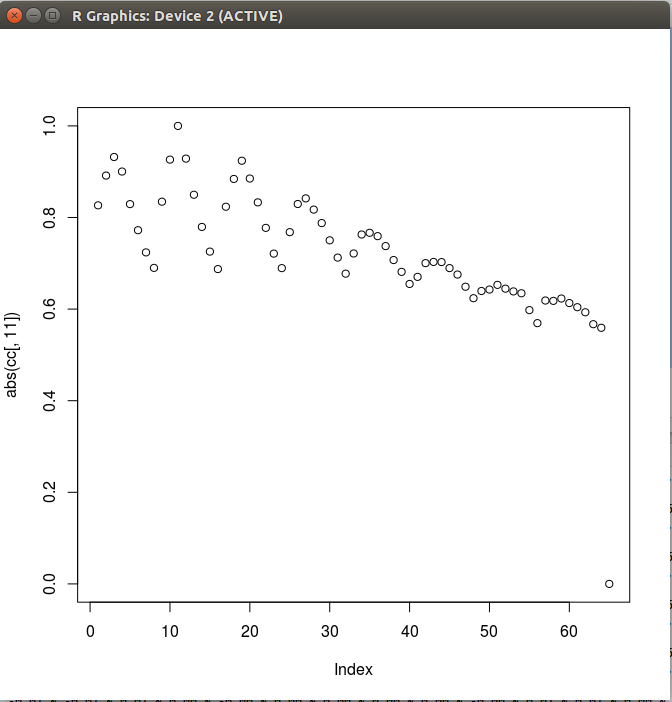
\includegraphics[width=5.0in]{yogurtplot1}
\caption{Decision tree for the yogurt dataset Script.}
\label{fig:dtyd}
\end{figure}

\begin{figure}[H]
\centering
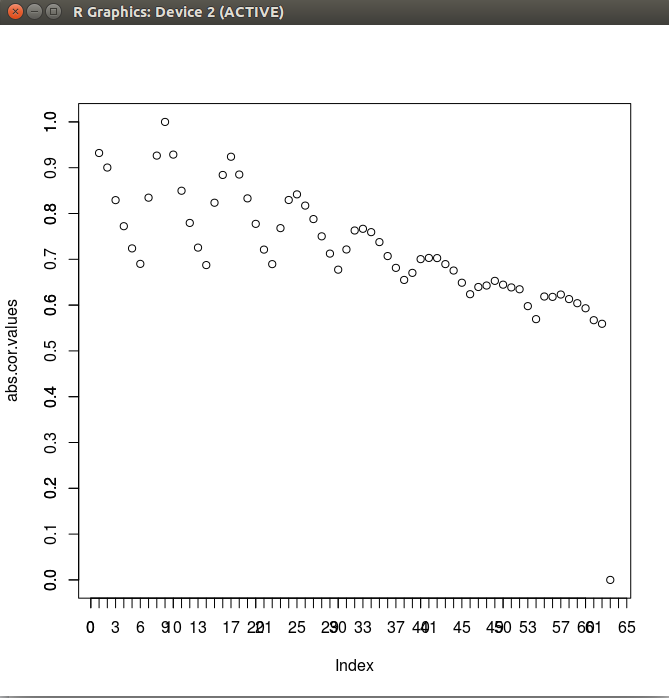
\includegraphics[width=5.0in]{yogurtplot2}
\caption{Decision tree for the yogurt dataset Script.}
\label{fig:dtyd}
\end{figure}

\begin{figure}[H]
\centering
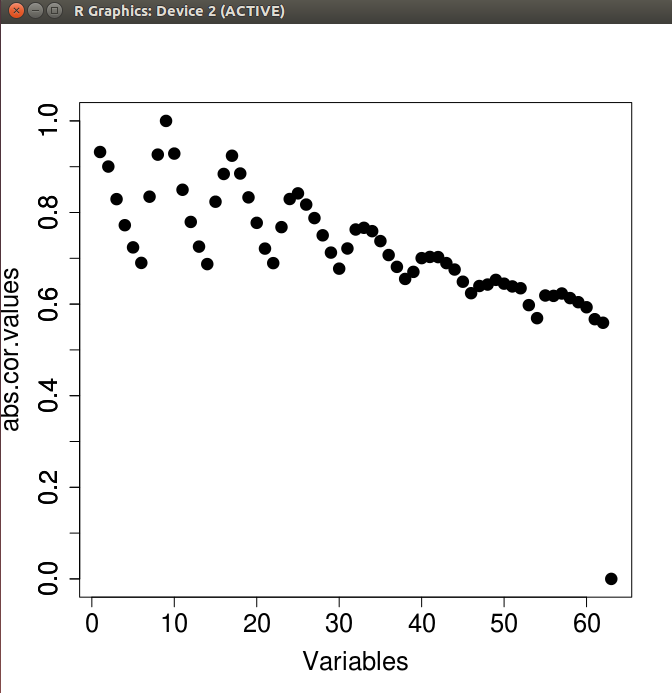
\includegraphics[width=5.0in]{yogurtplot3}
\caption{Decision tree for the yogurt dataset Script.}
\label{fig:dtyd}
\end{figure}

\begin{figure}[H]
\centering
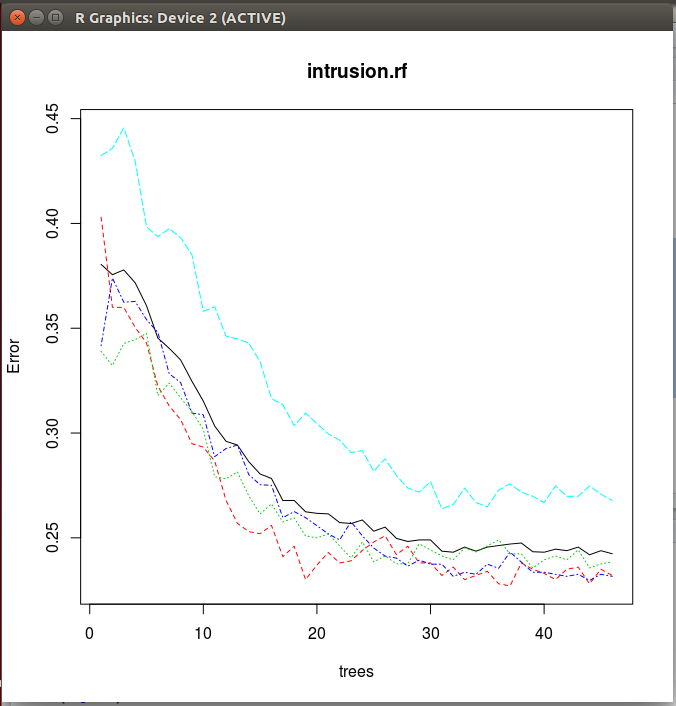
\includegraphics[width=5.0in]{yogurtplot5}
\caption{Decision tree for the yogurt dataset Script.}
\label{fig:dtyd}
\end{figure}

\begin{figure}[H]
\centering
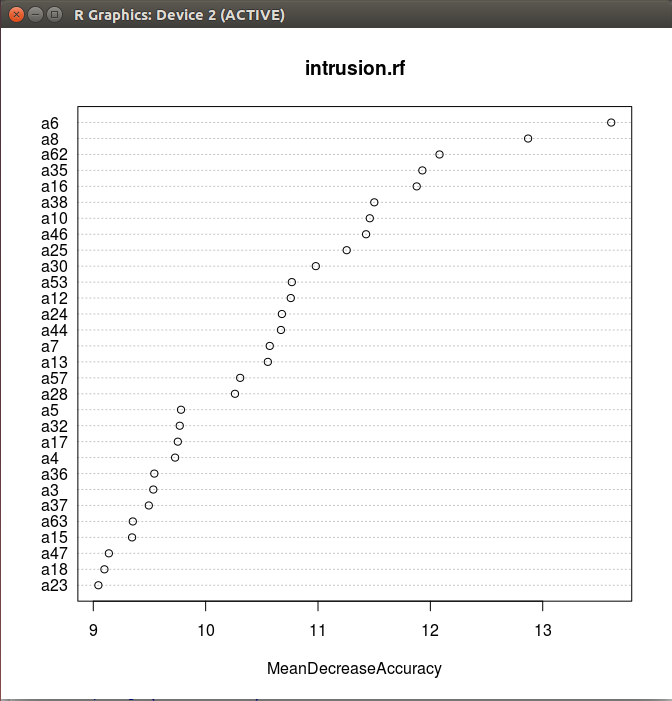
\includegraphics[width=5.0in]{yogurtplot6}
\caption{Decision tree for the yogurt dataset Script.}
\label{fig:dtcd}
\end{figure}

In the next three figures we will take a look at the random forest model's results of the yogurt dataset. Each of these figures have a different amount of trees, one is 250, one is 500, and the last is 1000. The differences between these trees should be substantial, however they're all within 1\% OOB estimate range of eachother.

\begin{figure}[H]
\centering
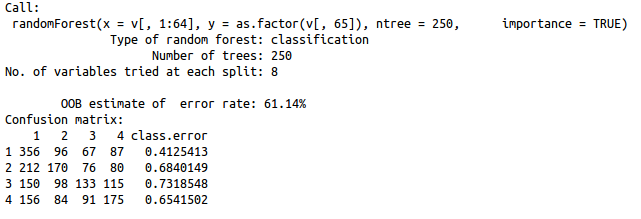
\includegraphics[width=5.0in]{yogurtOOB250}
\caption{OOB where ntree = 250.}
\label{fig:oob1}
\end{figure}

\begin{figure}[H]
\centering
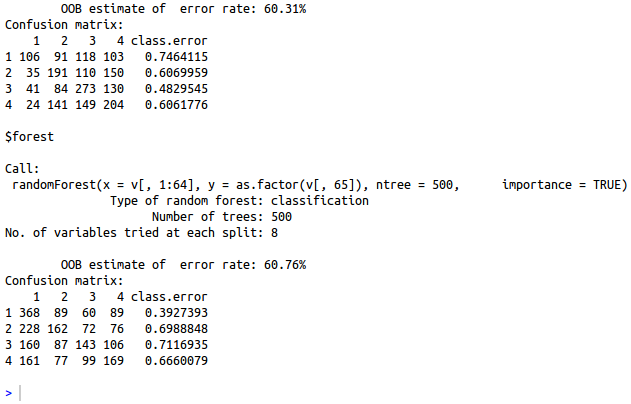
\includegraphics[width=5.0in]{yogurtOOB500}
\caption{OOB where ntree = 500.}
\label{fig:oob2}
\end{figure}

\begin{figure}[H]
\centering
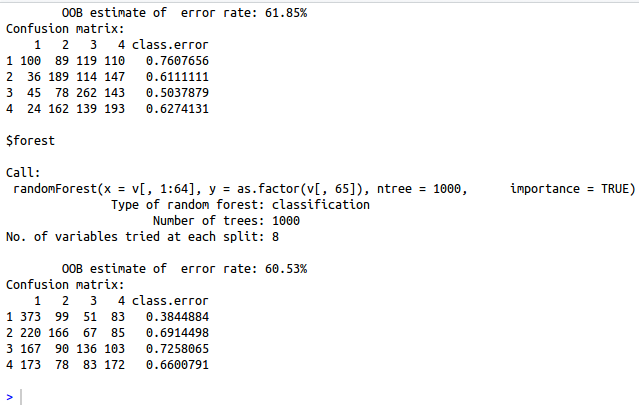
\includegraphics[width=5.0in]{yogurtOOB1000}
\caption{OOB where ntree = 1000.}
\label{fig:oob3}
\end{figure}

In the cat dataset the number of trees that produces the highest accuracy result was when ntree = 250. Here we can see that the highest accuracy given is when ntree = 1000. Our best accuracy is a whomping 60.53\%, a very undesirable score for this random forest algorithm. However, I can point out a few reasons why this machine is having trouble. The images were first reduced from full color images to grayscale images, then that image was stored as data. When these images are all grayscale, it's very hard for even a human to distinguish them. The gray colors look very similar, and even the shapes of the fruits at the bottom of the yogurt lid are nearly identical to each other. A higher number of trees does us more benefit so the machine can scrutinize every feature further.

\subsection{Conclusion}
Given a great number of levels of decisions, a random forest algorithm can have more success in a lower number of trees. If there are less levels of decision, a higher number of trees can help examine the feature more closely. However, when the observations are nearly identical there will still be a large margin of error. We found that with distinguishable enough data it is possible for this random forest based machine to differentiate between my cats.

\begin{thebibliography}{1}
\bibitem{bib:bogo}
K. Hong, \emph{BigData Single Node Cluster Hadoop Installation on Ubuntu}, http:\/\/www.bogotobogo.com\/Hadoop\/BigData\_hadoop\_Install\_on\_ubuntu\_single\_node\_cluster.php
\end{thebibliography}

\end{document}